\section{Implementation}

This section details the Implementation of OptiCaff and is located in the Google Code repository \footnote{\url{http://code.google.com/p/rich-2012-cafe/}}. The current to do items \footnote{\url{https://code.google.com/p/rich-2012-cafe/wiki/TODO}} and future work \footnote{\url{https://code.google.com/p/rich-2012-cafe/wiki/FutureWork}} are also located in the repository.

The external libraries used in the implementation of this project are located within the Appendix \ref{sec:Support}.

\subsection{Architecure}

The overall architecture of OptiCaff is shown in figure \ref{fig:Arch}.

\begin{figure}[ht]
\begin{center}
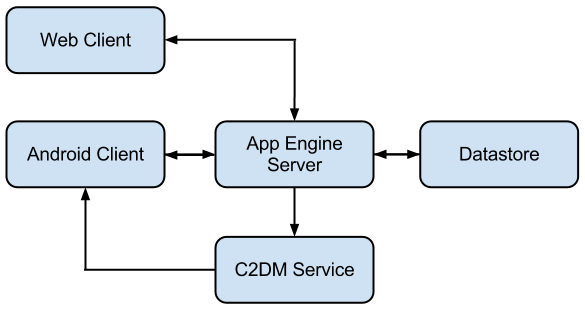
\includegraphics[trim = 0mm 0mm 0mm 0mm, clip, scale=0.4]{images/Architecture.png}
\caption{Architecture Diagram \cite{AppEngine}} 
\end{center}
\end{figure}

Google’s App Engine Connected Android Architecture \cite{AppEngine} which is based upon the client server model is used in OptiCaff. It allows OptiCaff to use a central database for storing caffeine related information which can be managed independently of open data sources. This removes the reliance on the providers of this data and explains why the results of the SPARQL queries that are run on the endpoints are stored. This also speeds up the process of delivering results to the users by not needing to perform these queries for every request. The specific advantages provided by this architecture are automatic handling of:

\begin{itemize}[noitemsep,leftmargin=1cm]
	\item{Communications between the service and the application.}
	\item{Authentication and user accounts.}
\end{itemize}

This also provides the means to notify users using Cloud to Device Messaging (C2DM).            

\subsection{Android}
This application has been developed for Android 4.0, Ice Cream Sandwich. OptiCaff was developed for this version due to the introduction of the official calendar API which is not in any previous versions of Android. This was necessary for OptiCaff to obtain a user’s event information. In addition to this, Ice Cream Sandwich is the first version of Android where Google have specified a recommended styling guide for designing applications.

OptiCaff is structured using the MVC design pattern, this allowed the packaging of the application code into various components which could then be worked on by different individuals independently and concurrently.                                                          

\subsection{User Interface}
                   
This section details the design considerations that were made prior to constructing the user interface.
                   
\subsubsection{Design Considerations}
When implementing the user interface, it was desirable that the design of the application was consistent with the Android 4.0 design ideology. To achieve this, the Android design and style guide was referenced, which outlines some of the key aspects of an Android 4.0 application, and some of Google’s design decisions made throughout the OS. This included decisions such as universal behaviour of the back button, should preferences be handled using a separate fragment or activity, and interaction and navigation of the different sub-activities of our application.
                   
Later versions of Android make use of an action bar which is implemented across all Android 4.0 applications as a way of providing a consistent method for navigation. This has therefore been included within OptiCaff with a main logo and icons which can be used to navigate between the different viewpoints.
                   
The user interface was designed so there were different activities for the different viewpoints available. There was one main activity for the home screen, and then activities for the map, graph, leaderboard, and the settings were implemented using the newer preference fragment class, which would match the preferences theme of the system. The ``Up” navigation option was implemented only on settings, as it is the only part of the application that is not a top level activity. Therefore all of the other activities make use of the back navigation instead, due to the lack of a hierarchy between the different viewpoints. Tapping on the OptiCaff logo in the top left corner will always take you back to the default home view.
                   
There are certain key design principles that have been outlined by Google in their style guide, that have been implemented in OptiCaff. Making sure that the important information is easily accessible, and the most important options and features can be accessed from the main home screen, providing an overview of events and the next time they should take caffeine. In the app structure they stress how the main home view should not just be a navigation menu, but instead stating the importance of ``making content the centerpiece of your start screen”, which this satisfies.       
                   
\subsubsection{Final Design}
                   
Figure \ref{fig:Activities} details the main screens of each activity section in Opticaff.
                   
\begin{figure}[ht]
\begin{center}
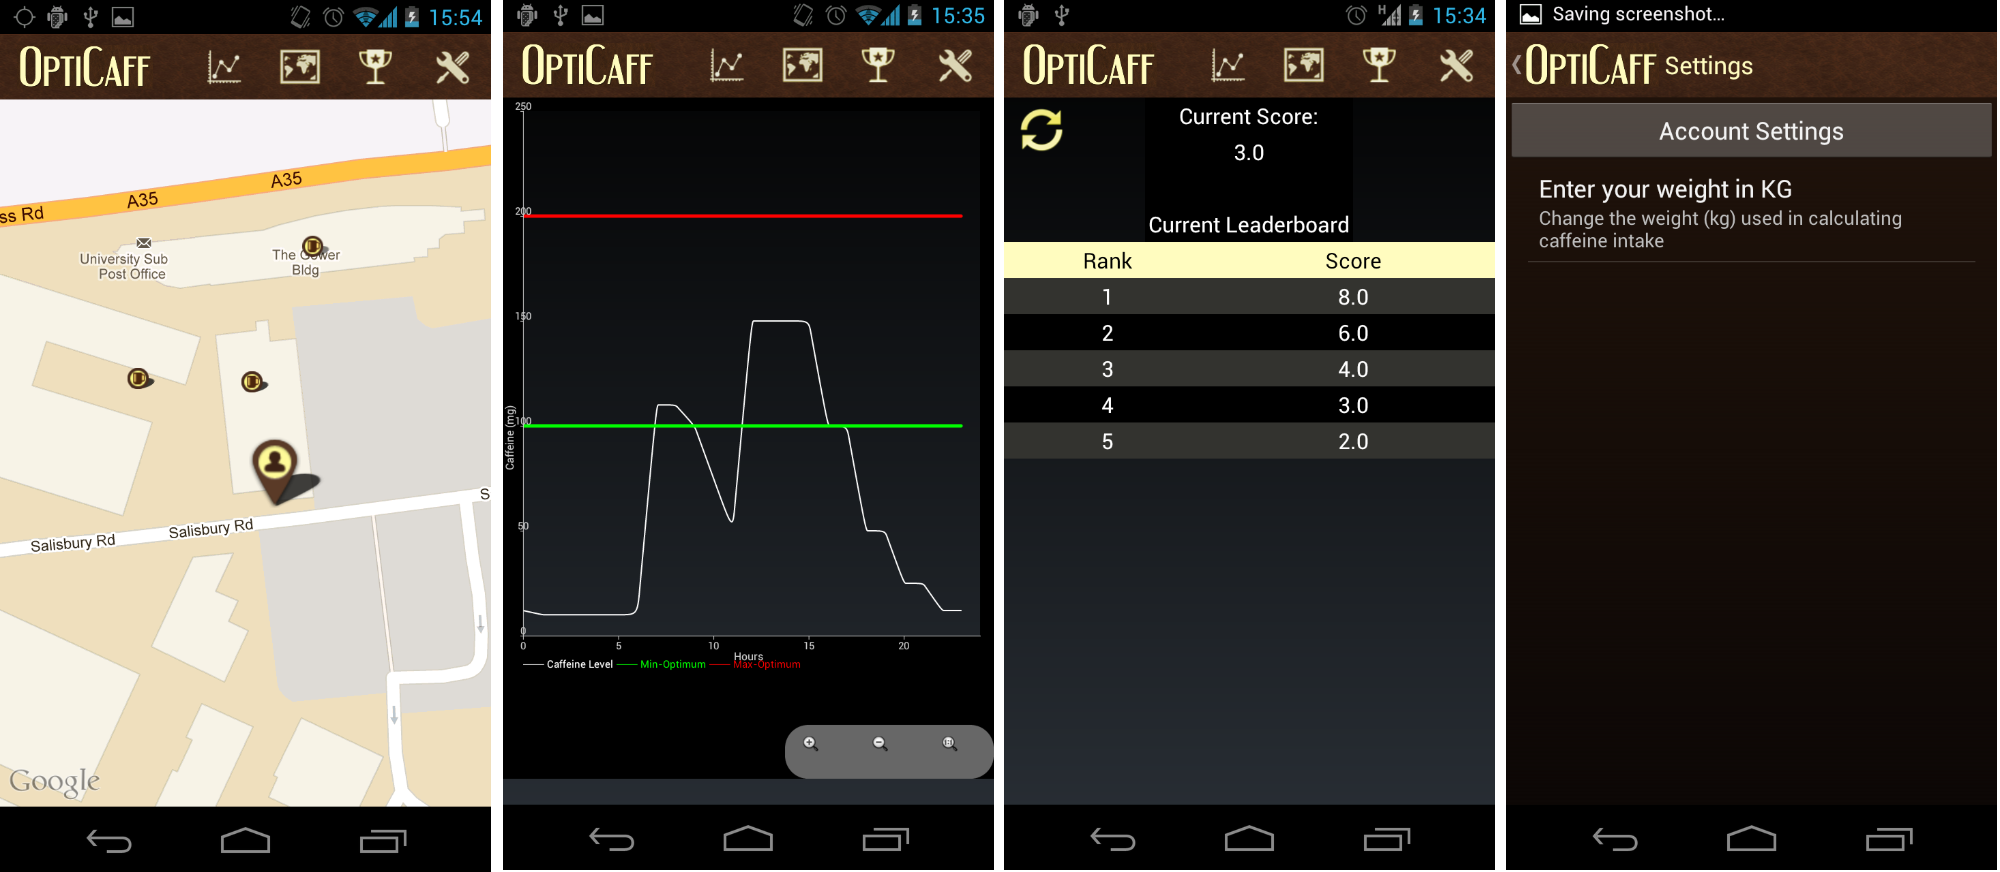
\includegraphics[scale=0.23]{images/app.png}
\caption{Activities: Maps, Graphs, Leaderboard \& Settings} 
\label{fig:Activities}
\end{center}
\end{figure}

\textbf{(a) Map Screen} \newline         
This screen uses the well known pointers utilised in popular map applications to illustrate the user’s location. The nearest caffeine vendors are shown in small brown circles around the map to give the user a visual idea of their proximity and direction.
                   
\textbf{(b) Graph Screen} \newline            
This screen shows the user’s caffeine levels over time throughout the day. This enables the user to easily see if they are staying within their optimal levels. The colours red and green are used to signal the minimum and maximum boundaries of the user’s optimum caffeine range. The colours used in the representation of the user’s optimum range (minimum and maximum line) follow a universal concept of red meaning bad and green meaning good.
                   
\textbf{(c) Leaderboard Screen} \newline     
This screen allows the user to see their current score and to compare it with other using the application. Putting the user’s score at the top in large text allows them to immediately assess whether they are achieving a good score through the use of positive and negative symbols.
                   
\textbf{(d) Settings Screen} \newline  
This screen allows users to change their settings. It is currently very simplistic as the prototype required minimal settings. The available settings provide a description of what each setting does and where possible an example value and user entered validation (i.e. the weight setting allows only positive numbers to be entered).

\subsection{Google App Engine}      
The GAE backend was implemented in Java and is split into a number of components: the Datastore and Remote Procedure Call (RPC) service. This decision was made due to the framework demanding the use of Google App Engine, which members of the team had previous experience using before and provided a free globally accessible data server which can be used by clients.
                       
\subsubsection{Datastore}
The first component is the database, which is implemented using GAE’s iteration of Java Data Objects (JDO). See Appendix \ref{sec:DataStore} for the structure of the datastore. The JDO datastore is used because it allows both the Android application and datastore to use the same Java objects and provides the means to transfer and use data easily.
                   
\subsubsection{RPC Service}       
The RPC service acts as an interface to the datastore for the Android Application.     This service contains a number of RPC methods which perform query actions on the datastore to provide information such as top 5 players on the leaderboards, and nearest caffeine source locations. This has been used because it provides an abstract interface between the client software and the datastore which handles authentication automatically.
               
                   
\subsection{Implementation Issues}
When developing the UI, the different activities were initially implemented in ‘fragments’, with one main container activity managing all of them. Unfortunately this caused issues when the map was implemented, as due to some incompatibilities between the MapActivity class in android and the new Fragment classes, there were problems when trying to contain what was viewed as an activity, within a fragment. This meant that different parts of OptiCaff were implemented as different activities.                           